%-------------------------------------------------------------------------------
%                            BAB II
%               TINJAUAN PUSTAKA DAN DASAR TEORI
%-------------------------------------------------------------------------------
\fancyhf{}
\fancyfoot[C]{\thepage}
\chapter{TINJAUAN KEPUSTAKAAN}

\par Untuk mendukung penelitian ini, maka dalam bab ini akan dikemukakan beberapa rumusan teori pendukung yang dikutip dari berbagai referensi baik dalam bentuk buku, jurnal, maupun tulisan karya ilmiah lainnya termasuk hasil penelitian sebelumnya yang ada kaitannya dengan penelitian yang dilakukan.

\section{\textit{MACHINE LEARNING}}
Teknologi \textit{machine learning} (ML) adalah mesin yang belajar atau dilatih dengan menggunakan algoritma dan data tertentu sehingga mesin bisa belajar sendirinya tanpa arahan pengguna. Pembelajaran mesin ini dikembangkan berdasarkan ilmu lainnya seperti statistika, matematika dan \textit{data mining} sehingga mesin dapat belajar dengan menganalisa data tanpa perlu diperintah oleh pengguna. Dalam hal ini \textit{machine learning} dapat memperoleh data yang ada dengan perintah ia sendiri. \textit{Machine learning} juga dapat mempelajari data yang ada dan data yang ia peroleh sehingga bisa melakukan tugas tertentu. Tugas yang dapat dilakukan oleh ML pun sangat beragam, tergantung dari apa yang ia pelajari \citep{Baker2019}.

\section{\uppercase{\textit{SUPERVISED LEARNING}}}
\textit{Supervised Learning} merupakan pendekatan pembelajaran mesin menggunakan set data yang berlabel. Kumpulan data ini dirancang untuk melatih atau "mengawasi" algoritma untuk mengklasifikasikan data atau memprediksi hasil secara akurat. Menggunakan input dan output berlabel, model dapat mengukur akurasinya dan belajar dari waktu ke waktu \citep{Gramejo2020}.

\par \textit{Supervised Learning} dibedakan menjadi dua jenis masalah yaitu klasifikasi dan regresi. Masalah klasifikasi menggunakan algoritma untuk secara akurat menentukan data uji ke dalam kategori tertentu, seperti memisahkan delima dari alpukat. Atau, di dunia nyata, algoritma pembelajaran yang diawasi dapat digunakan untuk mengklasifikasikan spam dalam folder terpisah dari kotak masuk Anda.

\section{\uppercase{\textit{CROWDSOURCING}}}
\textit{Crowdsourcing} adalah cara memperoleh layanan, ide, dan data berharga dari sekelompok orang, \textit{crowdsensing} adalah definisi yang sama hanya saja data diperoleh oleh perangkat atau sensor dan bukan dari input manusia. Sistem lokalisasi dalam ruangan berbasis Wi-Fi perlu membuat peta radio dengan survei lokasi. Proses survei lokasi memakan waktu dan \textit{crowdsourcing} adalah pilihan yang layak untuk mengatasi masalah ini. Sementara itu, perlindungan privasi telah menarik perhatian dari industri dan akademisi \citep{Li2018}.

\section{\uppercase{\textit{INDOOR LOCALIZATION SYSTEM} (ILS)}}
Teknologi ini merupakan layanan untuk menyediakan informasi bagi pengguna berdasarkan lokasi pengguna di suatu ruangan di dalam sebuah gedung, dinamakan \textit{Indoor Localization System}. \textit{Indoor Localization System} merupakan suatu sistem yang dapat menentukan lokasi \textit{smartphone} yang dimiliki setiap individu di dalam ruangan. Banyak penelitian yang telah dilakukan, yaitu implementasi \textit{Indoor Localization System} dengan menggunakan pemanfaatan WLAN. Namun, implementasi \textit{Indoor Localization System} dengan menggunakan pemanfaatan WLAN memiliki konsumsi daya baterai yang boros pada \textit{smartphone}. Pada akhirnya implementasi \textit{Indoor Localization System} diterapkan pada \textit{Bluetooth Low Energy }(BLE) yang memiliki konsumsi daya baterai \textit{smartphone} yang lebih murah. Terdapat tiga pendekatan dalam \textit{Indoor Localization System}, yakni berdasarkan jarak (trilaterasi), berdasarkan sudut (triangulasi) dan \textit{fingerprinting}. Metode yang digunakan pada penelitian ini adalah metode \textit{fingerprinting} \citep{Santos2021}.
%-----------------------------------------------------------------------------%

%\section{\uppercase{CROWDSOURCING INDOOR LOCALIZATION SYSTEM}}

\section{\uppercase{\textit{FINGERPRINTING}}}

\textit{Fingerprinting} merupakan metode yang paling akurat dan populer dalam penggunaannya untuk pelacakan objek pada lingkungan dalam ruangan \citep{Yim2010}. Menurut \citep{Muhammad2018}, \textit{Fingerprinting} adalah teknik untuk menentukan lokasi dengan pemanfaatan \textit{Radio Signal Strength} (RSS) dari suatu \textit{Access Point} (AP). Metode ini memperhitungkan atenuasi karena kekuatan sinyal sering berubah-ubah. Setiap titik referensi dikumpulkan yang mengintegrasikan adanya penghalang antara \textit{receiver} dan \textit{transmitter} \citep{Yudha2018}. Transmitter untuk teknologi IPS yang ditujukan untuk WLAN disebut dengan AP, sedangkan transmitter untuk teknologi IPS yang ditujukan untuk \textit{Bluetooth Low Energy} (BLE) disebut dengan \textit{Beacon}. Menurut \citep{Yudha2018}, metode \textit{Fingerprinting} berbasis IPS ini melibatkan 2 tahap yang dapat dilihat pada Gambar \ref{fingerprinting}.
%\section{Indoor Localization}
%\textit{Indoor Localization} merupakan. Dalam beberapa tahun terakhir, teknik \textit{Indoor Localization} telah banyak dibahas dan diteliti. Pada dasarnya, biaya yang murah dan akurasi tinggi adalah dua tujuan utama yang terus dikejar para peneliti untuk sistem penentuan posisi dalam ruangan. Sistem penentuan posisi dengan metode trilaterasi menggunakan Wi-Fi dan metode Fingerprinting adalah \textit{hotspot} dalam penelitian penentuan posisi dalam ruangan\citep{}. Beberapa peneliti mendesain sebuah sistem penentuan posisi dalam ruangan dengan menggabungkan Wi-Fi dan teknologi Radio Frequency (RF) lainnya seperti Radio Frequency Identification (RFID) dan Bluetooth Low Energy (BLE) untuk meningkatkan akurasi\citep{}. Metode yang digunakan pada penelitian ini adalah Bluetooth \textit{Fingerprinting} yang merupakan gabungan dari metode trilaterasi.
%-----------------------------------------------------------------------------%



\fancyhf{}
\fancyfoot[R]{\thepage}

\begin{figure}[H]
	\centering
	\shadowbox
	{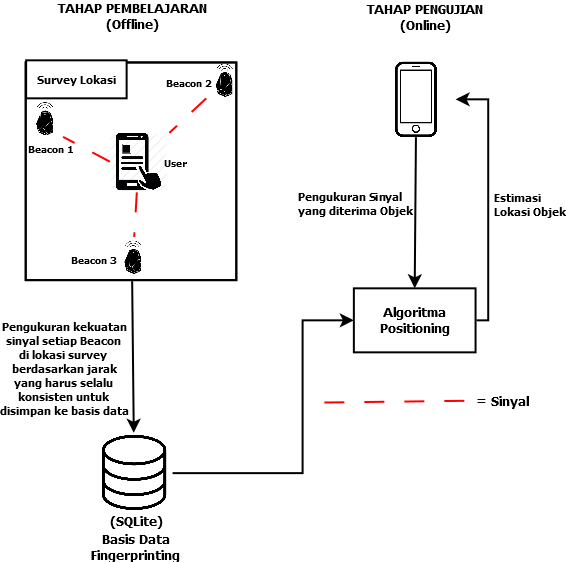
\includegraphics [width = 11cm, height= 9cm]{gambar/fingerprinting}}
	\caption{Ilustrasi Metode \textit{Fingerprinting} }.
	\label{fingerprinting}
\end{figure}

\par Tahap pertama adalah tahap pembelajaran (\textit{offline}), di mana lokasi \textit{Fingerprints} itu sendiri diperoleh dengan cara mengumpulkan RSSI dalam satuan desibel (dBm) yang dipancarkan dari masing-masing AP. Kemudian, gelombang radio akan dipancarkan oleh AP yang diletakkan pada posisi yang telah ditentukan sebelumnya ditangkap oleh \textit{smartphone} dengan kondisi WLAN ataupun Bluetooth dalam keadaan hidup. Selama tahap pembelajaran, lokasi yang tidak diketahui data pembelajarannya kemudian dirujuk sebagai titik referensi estimasi lokasi.
\newline
\par Tahap kedua adalah tahap pengujian (\textit{online}), di mana keakuratan perkiraan posisi objek sangat bergantung pada jumlah titik referensi yang dikumpulkan dalam data pembelajaran. Selama tahap pengujian, sistem harus memberikan informasi lokasi setiap objek berdasarkan data RSSI yang diamati. Namun, nilai RSSI bisa dipengaruhi oleh keadaan lingkungan sekitar yang dapat mengganggu keakuratannya.

\section{\uppercase{\textit{RECEIVED SIGNAL STRENGTH INDICATOR} (RSSI)}}
\textit{Positioning system} menghasilkan data yang penting untuk menghitung lokasi pengguna. \textit{Time of Arrival} (TOA), \textit{Time Difference of Arrival} (TDOA), \textit{Angle of Arrival} (AOA) dan RSSI adalah metode yang sesuai untuk menghitung data lokasi pengguna untuk kasus \textit{positioning system} \citep{Liu2007}. RSSI menunjukkan kekuatan atau daya yang diterima oleh sinyal \citep{Kajioka2014}. RSSI memperkirakan jarak \textit{node} yang belum diketahui ke referensi node dari beberapa kumpulan unit perhitungan dengan menggunakan atenuasi kekuatan sinyal (\textit{signal strength}) yang dipancarkan dari \textit{transmitter}. Metode ini tepat dilakukan dengan frekuensi sinyal radio \citep{Schneegans2007}.

\par Sebuah nilai RSSI didefinisikan dengan bilangan negatif. Semakin tinggi bilangan negatifnya, maka kekuatan sinyal tersebut tergolong lemah. Namun, jika bilangan nilai RSSI mendekati 0, maka kekuatan sinyal tersebut tergolong kuat. Biasanya, jika suatu objek berada di dekat AP atau \textit{transmitter}, RSSI akan memperoleh nilai yang besar. RSSI dapat digolongkan menjadi 5 kategori kekuatan sinyal seperti terlihat pada Tabel \ref{t_rssi}.

\begin{table}[H]
	\centering
	\caption{Kekuatan Sinyal RSSI \citep{VerisIndustries2013}}
	\label{t_rssi}
	\begin{tabular}{|l|l|l|}
		\hline
		\textbf{No.} & \textbf{Kekuatan Sinyal} & \textbf{Kualitas Sinyal} \\
		\hline
		1.           & Kurang dari -40 dB       & Luar Biasa               \\
		\hline
		2.           & -40 dB hingga -55 dB     & Sangat Baik              \\
		\hline
		3.           & -55 dB hingga -70 dB     & Baik                     \\
		\hline
		4.           & -70 dB hingga -80 dB     & Cukup Baik               \\
		\hline
		5.           & Lebih dari -80 dB        & Buruk                    \\
		\hline
	\end{tabular}
\end{table}

\section{\uppercase{\textit{BLUETOOTH LOW ENERGY} (BLE)}}
\par BLE \textit{Beacon} pada dasarnya adalah sebuah perangkat yang sangat sederhana berupa perangkat wireless kecil yang berbasiskan \textit{Bluetooth Low Energy} yang mentransmisikan sinyal radio secara terus menerus yang berkaitan dengan ID dari \textit{beacon} tersebut. Dengan menggunakan Smartphone Android terkini, BLE sangat mudah untuk dibaca dan dideteksi. Beberapa informasi yang diperoleh pada pembacaan ini, seperti data sensor dan estimasi jarak antara \textit{beacon} dengan Smartphone. Hanya dengan kedua data tersebut, developer dapat berkreasi untuk mengembangkan banyak aplikasi yang unik, aplikatif, dan dapat bermanfaat untuk optimasi sistem di industri juga manfaat lainnya \citep{Gupta2016}.

\par Meskipun BLE \textit{beacon} sangat sederhana, namun, BLE \textit{beacon} dibuat dengan teknologi yang cukup maju. Bluetooth Low Energy, yang merupakan media akses dari \textit{beacon}, memiliki cakupan yang cukup luas (Secara teori 200 m) dari segi jangkauan dibandingkan dengan Wireless Short Range lainnya. Bahkan saat ini dengan berkembangnya \textit{Bluetooth} 5.0, jangkauan \textit{Bluetooth Smart}, menurut Bluetooth SIG, dapat menjangkau 4 kali lipat dibandingkan dengan Bluetooth 4.0. Selain itu, dari sisi \textit{low energy}, teknologi ini menciptakan interaksi seamless yang tidak mengkonsumsi banyak energi baterai (secara teori, dengan baterai 3 volt dapat bertahan selama 2 tahun). Selain itu, oleh karena sistem yang tidak kompleks, teknologi \textit{beacon} tidak perlu bertarung dengan banyak standar aplikasi IoT, sehingga memudahkan developer dalam pengembangannya \citep{Gupta2013}.

\cite{Keluza2017}, mengemukakan bahwa Bluetooth merupakan alat komunikasi tanpa kabel yang digunakan untuk pertukaran data dalam jarak yang dekat. Bluetooth dikembangkan oleh Ericson di tahun 1994. Kemudian di tahun 1998 Ericson, IBM, Intel, Nokia dan Toshiba membentuk wewenang kekuasaan khusus yang dinamakan dengan Bluetooth Interest Group (SIG). Pertengahan tahun 2010, Bluetooth SIG mengumumkan spesifikasi dari Bluetooth 4.0, yang termasuk di dalamnya meliputi \textit{Bluetooth Classic}, \textit{Bluetooth High Speed} dan BLE. BLE terkadang juga bisa dikatakan sebagai “Bluetooth Pintar”. Meskipun BLE dan \textit{Bluetooth Classic} banyak memiliki kesamaan, BLE sebenarnya memiliki fungsionalitas yang sama sekali berbeda dari \textit{Bluetooth Classic}.

\par Keunggulan BLE dibandingkan \textit{Bluetooth Classic} adalah konsumsi daya baterai dan energi listrik dari BLE untuk \textit{transfer} data jauh lebih kecil dibandingkan dengan \textit{Bluetooh Classic}, tetapi dengan jangkauan konektivitas dan kapasitas pengiriman data yang sama \citep{bluetoothsig2010}. Karakteristik dari BLE adalah ukurannya yang sangat kecil, biaya murah, serta konsumsi daya rendah yang bisa digunakan sampai beberapa tahun ke depan dengan menggunakan jenis baterai AAA \citep{Keluza2017}. Menurut \cite{Paganini2015}, terdapat beberapa platform yang mendukung BLE dan platform tersebut sudah mendukung Bluetooth 4.0. Beberapa platform tersebut adalah sebagai berikut:
\begin {itemize}
\itemsep0em
\item iOS5+ (lebih dianjurkan iOS7+).
\item Android 4.3+ (perbaikan \textit{bug} merous di 4.4+).
\item Apple OS X 10.6+.
\item Windows 8 (XP, Vista dan Windows 7 hanya mendukung Bluetooth 2.1).
\item GNU/Linux Vanilla BlueZ 4.93+.
\end{itemize}

\section{\uppercase{\textit{BEACON}}}
\par Pada penelitian kali ini, \textit{beacon} yang digunakan adalah merk \textit{KBeacon}. \textit{Beacon} adalah teknologi \textit{Bluetooth Low-Energy} yang dapat digunakan untuk melakukan push notification atau tracking ketika kita sudah berada di jangkauan sinyalnya. Ketika pengguna melewati area di mana sistem penentuan posisi atau jaringan IoT dengan \textit{beacon} diatur, \textit{beacon} terdekat mengirimkan kode dengan pesan ke perangkat seluler mereka. Kemudian, pesan tersebut muncul sebagai pemberitahuan di perangkat seluler pengguna dengan aplikasi seluler pihak ketiga. Ada tiga hal yang harus diperhatikan untuk membuat sistem berbasis \textit{beacon} ini berfungsi, yaitu setidaknya ada satu perangkat \textit{beacon} lagi, aplikasi seluler dan tentunya izin pengguna. Untuk mengaktifkan dukungan \textit{beacon}, ponsel cerdas harus memiliki iOS 7 atau lebih tinggi atau Android 4 atau lebih tinggi. Standar \textit{beacon} Apple disebut \textit{iBeacon}, sedangkan Google bernama Eddystone \citep{Kim2014}.

\par BLE memancarkan sinyal dari alat \textit{transmiter} yang beroperasi menggunakan baterai. Alat \textit{transmiter} tersebut disebut dengan \textit{Beacon}. \textit{Beacon} merupakan alat pendeteksi lokasi dengan harga yang terjangkau, ukurannya yang kecil, memiliki daya tahan baterai yang cukup lama, dan tidak membutuhkan energi listrik tambahan. Setiap perangkat \textit{smartphone} dan \textit{tablets} yang mendeteksi sinyal dari \textit{Beacon}, dapat menghitung jarak dan memperkirakan keberadaan lokasi setiap perangkat sekaligus \citep{Keluza2017}.

\par Kelebihan dari penggunaan \textit{Beacon} diperkirakan bertahan sampai bertahun-tahun hanya dengan energi baterai, serta tahan terhadap debu dan air sesuai dengan standar IP67, dan memiliki ketelitian sejauh 1-3 meter \citep{Insoft2016}. Teknologi BLE merupakan solusi yang tepat yang digunakan pada \textit{Beacon}, karena penggunaan dayanya yang murah, BLE juga termasuk sistem yang ramah lingkungan. Penggunaan daya yang murah pada BLE dicapai dengan menjaga waktu proses transmisi data sesingkat mungkin dan mengizinkan perangkat \textit{smartphone} maupun \textit{tablets} berada pada mode tidur saat proses transmisi data \citep{Feng2011}.

\section{\uppercase{\textit{SUPPORT VECTOR MACHINE} (SVM)}}
\textit{Support vector machine} (SVM) adalah jenis algoritma klasifikasi \textit{supervised machine learning}. SVM pertama kali diperkenalkan pada 1960-an dan kemudian disempurnakan pada 1990-an. Namun, baru sekarang mereka menjadi sangat populer, karena kemampuan mereka untuk mencapai hasil yang cemerlang. SVM diimplementasikan dengan cara yang unik jika dibandingkan dengan algoritma pembelajaran mesin lainnya \citep{Campbell2010}.

\par Dalam kasus data yang dapat dipisahkan secara linier dalam dua dimensi, seperti yang ditunjukkan pada Gambar \ref{svm1}, algoritma pembelajaran mesin yang khas mencoba menemukan batas yang membagi data sedemikian rupa sehingga kesalahan klasifikasi dapat diminimalkan. Jika Anda melihat lebih dekat pada Gambar \ref{svm1}, mungkin ada beberapa batas yang membagi titik data dengan benar. Dua garis putus-putus serta satu garis padat mengklasifikasikan data dengan benar \citep{Zhibin2008}.

\begin{figure}[H]
	\centering
	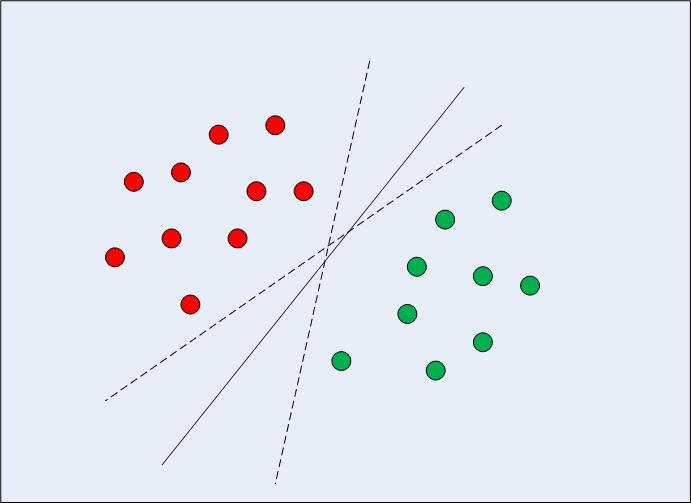
\includegraphics[width=11cm, height=8cm]{gambar/implementing-svm-kernel-svm-python-scikit-learn}
	\caption{Batas Keputusan Ganda.}
	\label{svm1}
\end{figure}

\par SVM berbeda dari algoritma klasifikasi lainnya dalam hal memilih batas keputusan yang memaksimalkan jarak dari titik data terdekat dari semua kelas. SVM tidak hanya menemukan batas keputusan; ia menemukan batas keputusan yang paling optimal.

\par Batas keputusan yang paling optimal adalah batas yang memiliki margin maksimum dari titik terdekat dari semua kelas. Titik terdekat dari batas keputusan yang memaksimalkan jarak antara batas keputusan dan titik disebut support vector seperti terlihat pada Gambar \ref{svm2}. Batas keputusan dalam kasus mesin support vector disebut \textit{maximum margin classifier}, atau \textit{maximum margin hyper plane}.

\begin{figure}[H]
	\centering
	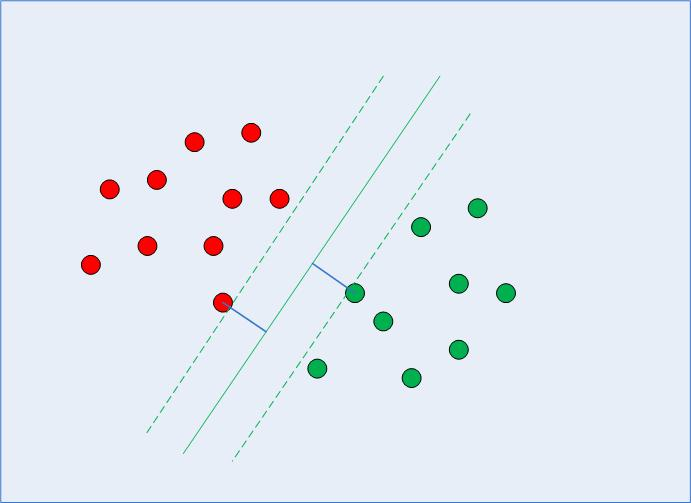
\includegraphics[width=11cm, height=8cm]{gambar/implementing-svm-kernel-svm-python-scikit-learn-2}
	\caption{Batas Keputusan dengan Support Vectors}
	\label{svm2}
\end{figure}

\par Margin (d) = minimum distance antara hyperplane and training samples. Hyperplane terbaik diperoleh dengan memaksimalkan d. Cara memaksimalkan d adalah :
\begin{equation}
	Margin = \frac{2}{|w|^2} = \frac{1-(-1)}{\sqrt{w{1}^2+w{2}}} = \frac{2}{|w|}
\end{equation}

Artinya meminimalkan:
\begin{equation}
	L(w)=\frac{|w|^2}{2}
\end{equation}

\par Umumnya, \textit{Support Vector Machines} dianggap sebagai pendekatan klasifikasi, tetapi dapat digunakan di kedua jenis masalah klasifikasi dan regresi. Itu dapat dengan mudah menangani beberapa variabel kontinu dan kategoris. SVM membangun hyperplane dalam ruang multidimensi untuk memisahkan kelas yang berbeda. SVM menghasilkan hyperplane optimal secara iteratif, yang digunakan untuk meminimalkan kesalahan. Ide inti dari SVM adalah untuk menemukan hyperplane marginal maksimum (MMH) yang paling baik membagi dataset ke dalam kelas \citep{Braun2011}.

\begin{figure}[H]
	\centering
	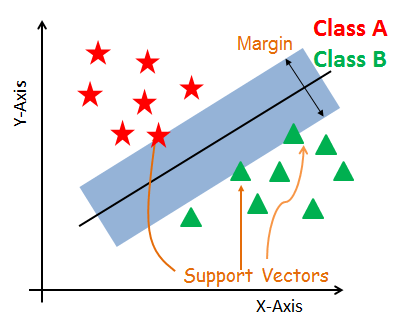
\includegraphics[width=10cm, height=7.3cm]{gambar/index3_souoaz}
	\caption{Support Vectors}
	\label{index3_souoaz}
\end{figure}

\par Support vector adalah titik data yang paling dekat dengan hyperplane. Titik-titik ini akan menentukan garis pemisah lebih baik dengan menghitung margin. Poin-poin ini lebih relevan dengan konstruksi classifier. Hyperplane adalah bidang keputusan yang memisahkan antara satu set objek yang memiliki keanggotaan kelas yang berbeda. Margin adalah jarak antara dua garis pada titik kelas terdekat. Ini dihitung sebagai jarak tegak lurus dari garis untuk mendukung vektor atau titik terdekat. Jika margin lebih besar di antara kelas, maka itu dianggap margin yang baik, margin yang lebih kecil adalah margin yang buruk \citep{Campbell2010}.

\par Tujuan utamanya adalah untuk memisahkan dataset yang diberikan dengan cara terbaik. Jarak antara kedua titik terdekat dikenal sebagai margin. Tujuannya adalah untuk memilih hyperplane dengan margin maksimum yang mungkin antara support vector dalam dataset yang diberikan. SVM mencari hyperplane marginal maksimum dalam langkah-langkah berikut:

\begin{enumerate}[1.]
	\itemsep0em
	\item Generate hyperplanes yang memisahkan kelas dengan cara terbaik. Gambar sisi kiri menunjukkan tiga hyperplanes hitam, biru dan oranye. Di sini, biru dan oranye memiliki kesalahan klasifikasi yang lebih tinggi, tetapi hitam memisahkan dua kelas dengan benar.

	\item Pilih hyperplane kanan dengan segregasi maksimum dari salah satu titik data terdekat seperti yang ditunjukkan pada gambar sisi kanan.
\end{enumerate}

\begin{figure}[H]
	\centering
	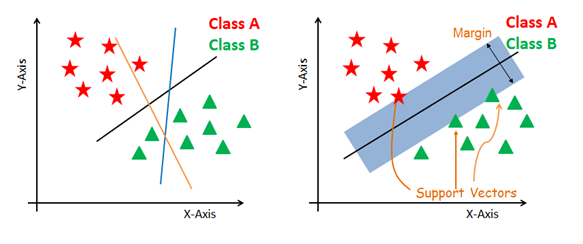
\includegraphics[width=14cm, height=6cm]{gambar/index2_ub1uzd}
	\caption{Support Vectors}
	\label{index3_souoaz}
\end{figure}
\par Beberapa masalah tidak dapat diselesaikan dengan menggunakan hyperplane linier, seperti yang ditunjukkan pada gambar di bawah (sisi kiri). Dalam situasi seperti itu, SVM menggunakan trik kernel untuk mengubah ruang input ke ruang dimensi yang lebih tinggi seperti yang ditunjukkan di sebelah kanan. Titik data diplot pada sumbu x dan sumbu z (Z adalah jumlah kuadrat dari $x$ dan $y$ : $z=x^2=y^2$)

\par Algoritma SVM diimplementasikan dalam praktik menggunakan kernel. Kernel mengubah ruang data input ke dalam bentuk yang diperlukan. SVM menggunakan teknik yang disebut trik kernel. Di sini, kernel mengambil ruang input berdimensi rendah dan mengubahnya menjadi ruang berdimensi lebih tinggi. Dengan kata lain, Anda dapat mengatakan bahwa itu mengubah masalah yang tidak dapat dipisahkan menjadi masalah yang dapat dipisahkan dengan menambahkan lebih banyak dimensi padanya. Hal ini paling berguna dalam masalah pemisahan non-linier. Trik kernel membantu Anda membuat pengklasifikasi yang lebih akurat \citep{Campbell2010}.
\begin{itemize}
	\itemsep0em
	\item Kernel linier dapat digunakan sebagai produk titik normal pada dua pengamatan yang diberikan. Produk antara dua vektor adalah jumlah perkalian dari setiap pasangan nilai input.

	      \begin{equation}
		      K(x, x_{i}) = \sum_{i=1}^{n} (x \times x{i})
	      \end{equation}

	\item Kernel polinomial adalah bentuk yang lebih umum dari kernel linier. Kernel polinomial dapat membedakan ruang input melengkung atau nonlinier.
	      \begin{equation}
		      K(X,X_{i})= 1 + \sum_{i=1}^{n} (X \times X{i})^d
	      \end{equation}

	      Dimana d adalah derajat polinomial. d=1 mirip dengan transformasi linier. Derajat perlu ditentukan secara manual dalam algoritma pembelajaran.

	\item Kernel Fungsi Basis Radial Kernel fungsi basis Radial adalah fungsi kernel populer yang umum digunakan dalam klasifikasi mesin vektor pendukung. RBF dapat memetakan ruang input dalam ruang dimensi tak terbatas.

	      \begin{equation}
		      K(x,x_{i}) = exp(-gamma \times \sum_{i=1}^{n} ((x – x{i}^2))
	      \end{equation}

	      Di sini gamma adalah parameter, yang berkisar dari 0 hingga 1. Nilai gamma yang lebih tinggi akan sangat cocok dengan dataset pelatihan, yang menyebabkan over-fitting. Gamma=0,1 dianggap sebagai nilai default yang baik. Nilai gamma perlu ditentukan secara manual dalam algoritma pembelajaran.
\end{itemize}


\section{\uppercase{ANDROID}}
Android adalah sistem operasi untuk perangkat \textit{smartphone} berbasis Linux \citep{Safaat2011}. Android menyediakan platform \textit{open source} bagi para \textit{developer} untuk menciptakan aplikasi mereka sendiri untuk digunakan oleh bermacam peranti bergerak. Aplikasi Android ditulis dengan bahasa pemrograman Java. Bagaimanapun juga, tanpa menggunakan standar Java Virtual Machine (JVM) sebuah aplikasi Android tidak akan bisa berjalan. Android SDK menyediakan sebuah \textit{tools} dan API untuk mengembangkan sebuah aplikasi pada platform \citep{Sarkar2019}. Menurut \cite{Supardi2011}, ada 4 komponen utama pada aplikasi Android yaitu sebagai berikut:
\begin{enumerate}[1.]
	\itemsep0em
	\item \emph{Activities}, merupakan komponen untuk menyajikan tampilan aplikasi kepada pengguna (\textit{user interface}).
	\item \emph{Service}, merupakan komponen yang tidak memiliki \textit{user interface} atau disebut dengan \textit{layout} pada Android. Namun, \textit{service} ini bekerja dengan cara \textit{background processing}.
	\item \emph{Broadcast Receiver}, merupakan komponen yang berfungsi menerima dan bertugas untuk menyampaikan notifikasi.
	\item \emph{Content Provider}, merupakan komponen yang menangani data secara spesifik sehingga dapat digunakan oleh aplikasi lain.
\end{enumerate}

\section{\uppercase{REACT NATIVE}}
React Native adalah framework JavaScript untuk mengembangkan aplikasi mobile secara multi-platform. Khususnya, pada bagian \textit{front-end} alias interface aplikasi. Sifatnya yang cross-platform memungkinkan satu codebase bisa digunakan di iOS dan Android. Selain itu, React Native juga menghasilkan aplikasi dengan UI/UX mengesankan. Aplikasi bisa berfungsi dengan \textit{smooth} dan komponennya (seperti tombol-tombol) merespon dengan baik layaknya dibuat dengan kode Native \citep{Brito2018}. Cara Kerja React Native cukup simple, yaitu:
\begin{enumerate}[1.]
	\itemsep0em
	\item Developer menggunakan kode React untuk membangun interface aplikasi
	\item Kode React akan diinterpretasikan menjadi JavaScript agar nantinya bisa digunakan untuk aplikasi mobile
	\item React Native akan menggunakan fitur bridge untuk mengolah codebase menjadi Native Module (Android Module, iOS Module)
	\item Native Module siap digunakan di platform yang bersangkutan.
\end{enumerate}

\section{\uppercase{WEB SERVICES}}
\par Web service merupakan aplikasi yang berisi sekumpulan basis data (database) dan perangkat lunak (software) atau bagian dari program perangkat lunak yang diakses secara remote oleh piranti dengan perantara tertentu. Melalui web service, memungkinkan pengguna untuk mengatasi permasalahan berupa interoperability dan mengintegrasikan sistem berbeda \citep{Chuangwei2011}.

\par Pada umumnya, web service memiliki ciri khusus berupa URL layaknya web. Yang membuat berbeda adalah interaksi yang diberikan oleh web service itu sendiri. URL pada web service hanya mengandung sekumpulan informasi, perintah, dan konfigurasi (sintaks yang berguna untuk membangun fungsi tertentu dari aplikasi). Web service mampu menukar data tanpa memandang sumber database, bahasa yang digunakan, dan pada platform apa data tersebut dikonsumsi. Kemampuan itulah yang memungkinkan web service menjadi jembatan penghubung untuk berbagai sistem \citep{Chuangwei2011}.

\par \textit{Web services} menggambarkan aplikasi yang mengekspos \textit{business logic} sebagai layanan yang menggunakan internet \citep{Mironela2009}. Layanan tersebut dikirim melalui \textit{interface} yang dapat diprogram, sementara fungsionalitasnya dapat dipakai dan dipanggil melalui alamat \textit{Internet Protocol} (IP \textit{address}) \citep{Wagh2012}. \textit{Web services} sering dikategorikan sebagai komponen sistem perangkat lunak yang dirancang untuk mendukung interaksi antar sistem. \textit{Web services} menyediakan informasi atau data pada sistem lain untuk digunakan sebagai fasilitas yang membuat sistem dapat saling berinteraksi. Biasanya, data yang diberikan oleh \textit{web services} berupa data dalam bentuk format JavaScript Object Notation (JSON) atau eXtensible Markup Language (XML) \citep{Rahman2013}. Situs \textit{web} World Wide Web Consortium (W3C) mendeskripsikan  bahwa \textit{Simple Object Access Protocol} (SOAP), \textit{Representatonal State Transfer} merupakan protokol yang digunakan \textit{web services} untuk berkomunikasi. Penelitian ini akan menggunakan \textit{web services} dengan layanan protokol REST untuk membantu aplikasi absensi perkuliahan berbasis Android berinteraksi dengan \textit{database} yang terdapat di server.

\section{\uppercase{REPPRESENTATIONAL STATE TRANSFER (REST)}}
REST merupakan hubungan antara klien dan server dan bagaimana sebuah data disimpan. Arsitektur REST didasarkan pada gaya arsitektur klien atau server yang dapat dilihat pada Gambar \ref{restful}. \textit{Request} dan \textit{response} dibangun berdasarkan sumber daya pada saat proses transfer \citep{HaliliRamadani2018}. Konsep dari REST adalah perpindahan antar \textit{state}, dapat dicontohkan seperti sebuah browser yang melakukan permintaan terhadap sebuah halaman situs, maka server akan mengirimkan \textit{state} dari halaman situs tersebut ke browser \citep{Rahman2013}.
\begin{figure}[H]
	\centering
	\shadowbox
	{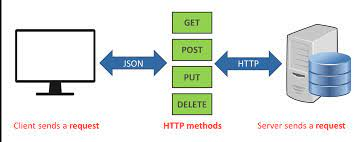
\includegraphics [width = 11cm, height= 4cm]{gambar/restful.jpg}}
	\caption
	{Ilustrasi Arsitektur RESTful dan Komunikasi Antara Klien dan Server \citep{HaliliRamadani2018}}.
	\label{restful}
\end{figure}
\par Navigasi REST dilakukan melalui HTTP untuk melakukan aktivitas tertentu, seolah-olah terjadi perpindahan \textit{state} antara satu halaman dengan halaman lainnya \citep{Rahman2013}. Sebuah aplikasi \textit{web} yang bergantung dengan layanan REST arsitektur disebut dengan RESTful \textit{web services}. RESTful \textit{web services} menggunakan 4 perintah HTTP untuk \textit{create}, \textit{read}, \textit{update} dan \textit{delete} yaitu \textit{GET}, \textit{POST}, \textit{PUT} dan \textit{DELETE} seperti yang terlihat pada Gambar \ref{httprestful} \citep{sinha2014}.
\begin{figure}[H]
	\centering
	\shadowbox
	{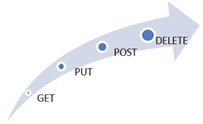
\includegraphics [width = 5cm, height= 3cm]{gambar/httprestful}}
	\caption{Perintah HTTP RESTful \citep{sinha2014}}.
	\label{httprestful}
\end{figure}

\section{\uppercase{SCRUM}}

\par Scrum adalah metode pengembangan perangkat lunak \textit{agile} yang dikembangkan oleh Jeff Sutherland dan tim pengembangannya di awal 1990-an. Selanjutnya, pengembangan lebih lanjut tentang metode Scrum telah dilakukan oleh Schwaber dan Beedle Prinsip scrum konsisten dengan manifesto agile dan digunakan untuk memandu kegiatan pengembangan dalam suatu proses yang menggabungkan kegiatan kerangka kerja (\textit{framework activity}) berikut: kebutuhan (\textit{requirements}), analisis (\textit{analysis}), desain (\textit{design}), evolusi (\textit{evolution}), dan pengiriman (\textit{delivery}). Dalam setiap kegiatan kerangka kerja, \textit{work task} terjadi dalam pola proses yang disebut \textit{sprint}. Pekerjaan yang dilakukan dalam \textit{sprint} (jumlah \textit{sprint} yang diperlukan untuk setiap kegiatan kerangka kerja akan bervariasi tergantung pada kompleksitas dan ukuran produk) disesuaikan dengan masalah yang dihadapi dan didefinisikan dan sering dimodifikasi secara real time oleh tim Scrum \citep{Ereiz2019}.

\par \textit{Scrum} pada dasarnya didasari oleh proses model \textit{Incremental} yang merupakan salah satu model pengembangan perangkat lunak. Dalam metode \textit{Scrum}, seluruh \textit{development cycle} terbagi menjadi sebuah rangkaian iterasi di mana setiap iterasi tersebut merupakan detak jantung dari \textit{Scrum} itu sendiri yang disebut dengan “\textit{Sprint}”. Pengerjaan \textit{Sprint} memiliki durasi maksimal selama 30 hari. Karena durasi \textit{Sprint} lebih singkat dibandingkan dengan durasi pengembangan produk, maka dalam produk \textit{development cycle} akan ada beberapa \textit{Sprint}, yang artinya pengembangan produk dengan metode \textit{Scrum} dilakukan secara \textit{Iterative} dan \textit{Incremental} \citep{Mundra2013}. Tahapan-tahapan metode \textit{Scrum} menurut \cite{Schwab2013} adalah sebagai berikut:
\begin {enumerate}[1.]
\item Dimulai dengan mengumpulkan \textit{user requirements}, namun tidak harus semua \textit{requirements} diharapkan harus keluar dari pemikiran \textit{user} di tahap awal proses pengembangan. \textit{User} dapat mengubah pikiran mereka di setiap waktu selama proses pengembangan, \textit{user} dapat menambah fitur-fitur baru, menghapus atau memperbarui beberapa fitur yang telah ada sebelumnya.
%%%%%%%%%%%%%%%%%%%%%%%%%%%%%%%%%%%%%%%%%%%%%%%%%%%%%%%%%%%%%%%%%%%%%%%%%%%%%%%%%%%%%%%%%%%%%%%%%%%%%%%%%
\item Tahapan selanjutnya adalah memprioritaskan \textit{requirements} dan \textit{Product Backlog}. Sebuah perencanaan yang tepat dalam \textit{Sprint} harus dilakukan sesuai jumlah \textit{Sprint} yang dibutuhkan untuk mengembangkan perangkat lunak, yang terdiri dari durasi \textit{Sprint} tersebut dan \textit{requirements} apa saja yang terdapat di \textit{Product Backlog} yang harus diimplementasikan di setiap \textit{Sprint} (dikenal dengan \textit{Sprint Backlog}).
%%%%%%%%%%%%%%%%%%%%%%%%%%%%%%%%%%%%%%%%%%%%%%%%%%%%%%%%%%%%%%%%%%%%%%%%%%%%%%%%%%%%%%%%%%%%%%%%%%%%%%%%%
\item \textit{Sprint} diawali dengan \textit{Sprint Planning} dimana \textit{Product Owner}, satu orang yang telah diberikan wewenang dan bertanggung jawab untuk memaksimalkan nilai produk di pasar, bertemu dengan tim \textit{Scrum} (tim dengan jumlah 2-9 orang), kemudian bekerja sama untuk memperkirakan \textit{requirements} dari \textit{Product Backlog} apa saja yang dikerjakan selama satu \textit{Sprint}.
%%%%%%%%%%%%%%%%%%%%%%%%%%%%%%%%%%%%%%%%%%%%%%%%%%%%%%%%%%%%%%%%%%%%%%%%%%%%%%%%%%%%%%%%%%%%%%%%%%%%%%%%% 
\item \textit{Sprint Planning} difasilitasi dengan \textit{Scrum Master}. \textit{Scrum Master} adalah seorang pemimpin yang melayani (\textit{Servant Leader}). \textit{Sprint Planning} memiliki batasan waktu selama 8 jam di dalam sebuah \textit{Sprint} yang berdurasi selama 30 hari. Keluaran dari \textit{Sprint Planning} adalah daftar pekerjaan dari hasil kesepakatan antara \textit{Product Owner} dan tim \textit{Scrum} dimana pekerjaan itu yang akan dikerjakan oleh tim \textit{Scrum} nantinya selama satu \textit{Sprint} beserta \textit{Sprint Goal} yang dinamakan dengan \textit{Sprint Backlog}.
%%%%%%%%%%%%%%%%%%%%%%%%%%%%%%%%%%%%%%%%%%%%%%%%%%%%%%%%%%%%%%%%%%%%%%%%%%%%%%%%%%%%%%%%%%%%%%%%%%%%%%%%%
\item Setelah \textit{Sprint Planning} berakhir, tim \textit{Scrum} akan mengambil \textit{Sprint Backlog} untuk diri mereka masing-masing dan mengerjakan \textit{Sprint Backlog} setiap hari hingga akhir \textit{Sprint} tanpa campur tangan dari pihak manapun. \textit{Daily Scrum} akan dikerjakan oleh tim \textit{Scrum} yang tidak lebih dari 15 menit untuk menentukan apa saja yang akan mereka kerjakan selama 24 jam ke depan berdasarkan perkembangan 24 jam terakhir, serta menyampaikan permasalahan yang menghambat mereka untuk bisa mencapai \textit{Sprint Goal}. Tim \textit{Scrum} akan melakukan perbaikan-perbaikan item dari \textit{Product Backlog} pada \textit{Sprint} yang akan datang selama proses pengembangan berlangsung, dengan tujuan membuat \textit{Sprint Planning} menjadi lebih efektif.
%%%%%%%%%%%%%%%%%%%%%%%%%%%%%%%%%%%%%%%%%%%%%%%%%%%%%%%%%%%%%%%%%%%%%%%%%%%%%%%%%%%%%%%%%%%%%%%%%%%%%%%%%
\item Di akhir \textit{Sprint} saat acara \textit{Sprint Review}, \textit{Product Owner} akan mempresentasikan hasil pekerjaan tim \textit{Scrum} selama satu \textit{Sprint} dan juga menjelaskan apa saja pencapaian tim \textit{Scrum} menuju \textit{Sprint Goal} di dalam \textit{Sprint} tersebut kepada para pemegang kepentingan (\textit{stakeholder}) agar mendapatkan \textit{feedback}. \textit{Feedback} ini akan dimasukkan ke dalam \textit{Product Backlog} agar meningkatkan nilai dari sebuah produk. \textit{Sprint Review} memiliki batasan waktu tidak lebih dari 4 jam untuk \textit{Sprint} yang memiliki durasi selama 30 hari.
%%%%%%%%%%%%%%%%%%%%%%%%%%%%%%%%%%%%%%%%%%%%%%%%%%%%%%%%%%%%%%%%%%%%%%%%%%%%%%%%%%%%%%%%%%%%%%%%%%%%%%%%%
\item Setelah \textit{Sprint Review}, \textit{Scrum Master} memfasilitasi acara yang bernama \textit{Sprint Retrospectives} agar tim \textit{Scrum}, \textit{Product Owner} bekerja sama menentukan apa saja peningkatan yang akan mereka implementasikan di \textit{Sprint} berikutnya. \textit{Scrum Master} yang efektif, akan kreatif dalam memfasilitasi \textit{Sprint Retrospectives}, akan masuk ke dalam \textit{Sprint Backlog} untuk menuju \textit{Sprint} berikutnya. \textit{Definition of Done} adalah salah satu hal yang ditekankan oleh tim \textit{Scrum} pada saat \textit{Sprint Retrospectives}.
%%%%%%%%%%%%%%%%%%%%%%%%%%%%%%%%%%%%%%%%%%%%%%%%%%%%%%%%%%%%%%%%%%%%%%%%%%%%%%%%%%%%%%%%%%%%%%%%%%%%%%%%%
\item \textit{Sprint Retrospectives} merupakan acara yang paling penting dalam \textit{Scrum} dikarenakan sifatnya yang menekankan \textit{continuous learning} yang dapat meningkatkan tingkat \textit{agility} perusahaan. \textit{Sprint Review} memiliki batasan waktu tidak lebih dari 3 jam untuk \textit{Sprint} yang memiliki durasi selama 30 hari. Setelah \textit{Sprint Retrospectives} berakhir, maka \textit{Sprint} berikutnya akan langsung dilakukan tanpa ada jeda antar \textit{Sprint}. Pada setiap \textit{Sprint}, \textit{Product Owner} akan memastikan agar produk dapat mencapai nilai setinggi mungkin saat pengembangan produk diakhiri. \textit{Product Owner}, \textit{Scrum Master} dan tim \textit{Scrum} memegang komitmen, keberanian, saling menghargai satu sama lain, keterbukaan dan fokus. Ilustrasi tahapan-tahapan metode Scrum dapat dilihat pada Gambar \ref{scrum} dibawah ini.
\end{enumerate}

\vspace{0,2cm}
\begin{figure}[H]
	\centering
	\shadowbox
	{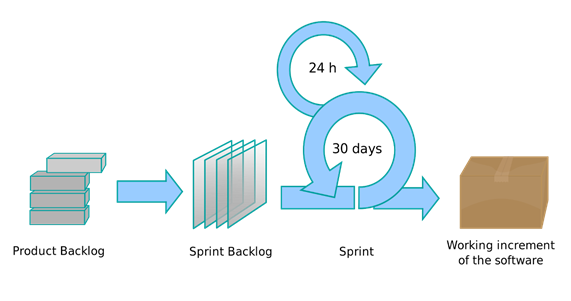
\includegraphics [width = 11cm, height= 5.5cm]{gambar/imagescrum}}
	\caption{Ilustrasi Metode Pengembangan Menggunakan \textit{Scrum} \citep{Schwab2013}}.
	\label{scrum}
\end{figure}


\section{\uppercase{BLACK BOX TESTING}}
Pengujian \textit{black-box} adalah metode pengujian perangkat lunak yang memeriksa fungsionalitas aplikasi tanpa mengintip ke dalam struktur atau cara kerja internalnya. Metode pengujian ini dapat diterapkan secara virtual ke setiap tingkat pengujian perangkat lunak: unit, integrasi, sistem, dan penerimaan. Kadang-kadang disebut sebagai pengujian berbasis spesifikasi. \textit{Black box testing} menurut \citep{Mustaqbal2015} cenderung menemukan hal-hal berikut:
\begin{enumerate}[1.]
	\item Fungsi yang tidak benar atau tidak ada.
	\item Kesalahan \textit{user interface}.
	\item Kesalahan pada struktur data dan akses \textit{database}.
	\item Kesalahan performansi.
	\item Kesalahan inisialisasi dan terminasi.
\end{enumerate}

\section{\uppercase{USABILITY TESTING}}
\par Pengujian kegunaan adalah teknik yang digunakan dalam desain interaksi yang berpusat pada pengguna untuk mengevaluasi suatu produk dengan mengujinya pada pengguna. Ini dapat dilihat sebagai praktik kegunaan yang tak tergantikan, karena memberikan masukan langsung tentang bagaimana pengguna sebenarnya menggunakan sistem. Ini lebih peduli dengan intuitif desain produk dan diuji dengan pengguna yang tidak memiliki paparan sebelumnya. Pengujian tersebut sangat penting untuk keberhasilan produk akhir sebagai aplikasi yang berfungsi penuh yang menciptakan kebingungan di antara penggunanya tidak akan bertahan lama.Ini berbeda dengan metode pemeriksaan kegunaan di mana para ahli menggunakan metode yang berbeda untuk mengevaluasi antarmuka pengguna tanpa melibatkan pengguna.
\citep{Wahl2000}.  \citep{Wesfix2017}.

\par Tujuan lain dilakukannya pengujian ini adalah untuk mengumpulkan data kualitatif yang berhubungan dengan kepuasan pengguna dengan produk yang diuji. Data kualitatif tersebut terdiri dari komentar yang dibuat oleh partisipan, jawaban dari kuesioner pertanyaan dan tanggapan dari partisipan saat proses wawancara. \textit{Usability testing} telah terbukti dapat mengurangi waktu tahap pengembangan, mengurangi jumlah \textit{bugs}, dan menghasilkan produk yang lebih berkualitas untuk meningkatkan nilai jual \citep{Wahl2000}.

\subsection{\textit{Usability Metric for User Experience} (UMUX)}
Metode pengujian dengan \textit{usablity testing} yang digunakan pada penelitian ini adalah UMUX. \textit{Usability Metric for User Experience} (UMUX) adalah sebuah skala Likert yang mempunyai 4 (empat) item yang digunakan untuk melakukan sebuah penilaian subjektif dari manfaat sebuah aplikasi. UMUX dibuat untuk menghasilkan hasil yang mirip dengan hasil yang diperoleh dengan skala \textit{system usability} yang memiliki 10 item. Selain itu, \textit{Usability Metric for User Experience} (UMUX) cukup ringkas untuk digunakan sebagai modul kegunaan dalam matriks \textit{user experience}. UMUX ditujukan untuk mencocokkan kinerja dari \textit{system usability scale} (SUS) dan penyesuaian dengan langkah-langkah yang lebih penting, UMUX dapat diberikan secara online sebagai survei atau sebagai tindak lanjut dalam pengujian kegunaan, UMUX juga mudah untuk dikelola, karena tidak memerlukan percabangan atau penataan ulang item \citep{Finstad2010}

% \subsection{System Usablity Scale (SUS)}
% Metode pengujian dengan \textit{usablity testing} yang digunakan pada penelitian ini adalah SUS. System Usability Scale (SUS) menyediakan alat yang "cepat dan kotor", andal untuk mengukur kegunaan. Ini terdiri dari 10 item kuesioner dengan lima pilihan respon untuk responden; dari Sangat setuju hingga Sangat tidak setuju. Awalnya dibuat oleh John Brooke pada tahun 1986, ini memungkinkan Anda untuk mengevaluasi berbagai macam produk dan layanan, termasuk perangkat keras, perangkat lunak, perangkat seluler, situs web, dan aplikasi.

% \par Skala penilaian yang digunakan yaitu skala likert antara 1-5. \cite{Sugiyono2004} mengatakan bahwa skala likert digunakan untuk mengukur pendapat, persepsi dan sikap seseorang atau sekelompok orang tentang fenomena sosial. SUS bertujuan untuk mengetahui penilaian subjektif yang dilakukan dalam pengujian oleh beberapa responden dan meminta pendapat mengenai aplikasi yang akan dibuat pada penelitian ini.

% \par Pengujian ini memerlukan kuesioner sebagai teknik pengumpulan informasi pengujian yang didapat dari responden mengenai aplikasi. Kuesioner terdiri dari 10 soal yang terdiri dari pertanyaan positif dan negatif. Pertanyaan positif terdapat pada nomor ganjil (1, 3, 5, 7, 9) dan pertanyaan negatif terdapat pada nomor genap (2, 4, 6, 8, 10). Setiap pertanyaan diberi bobot antara 0-4. Pertanyaan ganjil skor dihitung dengan cara bobot tiap pertanyaan ($x_{i}$) dikurangi 1 (ditulis $x_{i}$ - 1). Sedangkan pertanyaan genap skor dihitung dengan cara 5 dikurangi bobot tiap pertanyaan ($x_{i}$)(ditulis 5 - $x_{i}$) \citep{Ardiansyah2016}. Setiap pertanyaan memiliki 5 pilihan jawaban yang terdiri dari: sangat tidak setuju, tidak setuju, biasa saja, setuju dan sangat setuju.

%\par Rumus menghitung skor pengujian \textit{usability testing} adalah sebagai berikut:
%\begin{equation}
%\overline{x}=\frac{\sum x}{n}
%\end{equation}
%\newline
%Keterangan:\newline
%$\overline{x}$ = skor rata-rata. \newline
%$\sum x$ = jumlah skor SUS. \newline
%$n$ = jumlah responden. 

\subsection{Test Plan}
\textit{Test plan} adalah dokumen yang melibatkan semua anggota tim \textit{developer} untuk melihat apakah fungsionalitas dari produk yang dibuat sudah terpenuhi atau belum. Dengan kata lain, \textit{test plan} disebut sebagai tujuan, perencanaan atau skenario untuk melakukan \textit{testing} yang akan dilakukan baik itu \textit{expert} \textit{user} atau \textit{user} awam. \textit{Test plan} perlu dibuat saat melakukan pengujian karena \textit{test plan} menggambarkan bagaimana cara menguji produk tersebut. \textit{Test plan} memaksa untuk melakukan pengujian secara sistematis \citep{Rubin2008}. Bagian-bagian dari \textit{test plan} menurut \cite{Rubin2008} adalah sebagai berikut:
\begin{itemize}
	\item Maksud, tujuan dan sasaran pengujian.
	\item Pertanyaan terkait penelitian.
	\item Karakteristik partisipan.
	\item Metode yang digunakan (\textit{test design}).
	\item \textit{List} tugas.
	\item Lingkungan pengujian, perlengkapan, dan logistik.
	\item Peran moderator pengujian.
	\item Data yang dikumpulkan dan langkah-langkah evaluasi.
	\item Laporan dan presentasi.
\end{itemize}








%-----------------------------------------------------------------------------%

% Baris ini digunakan untuk membantu dalam melakukan sitasi
% Karena diapit dengan comment, maka baris ini akan diabaikan
% oleh compiler LaTeX.
\begin{comment}
\bibliography{daftar-pustaka}
\end{comment}
